\graphicspath{{./figures}}

\section{Software}
The following section documents notable choices made during implementation, but after design. All code is available at \url{https://github.com/gvcallen/pqcom/tree/main/code}.

\subsection{Mount Control}
\begin{figure}[!htb]
  \centering
  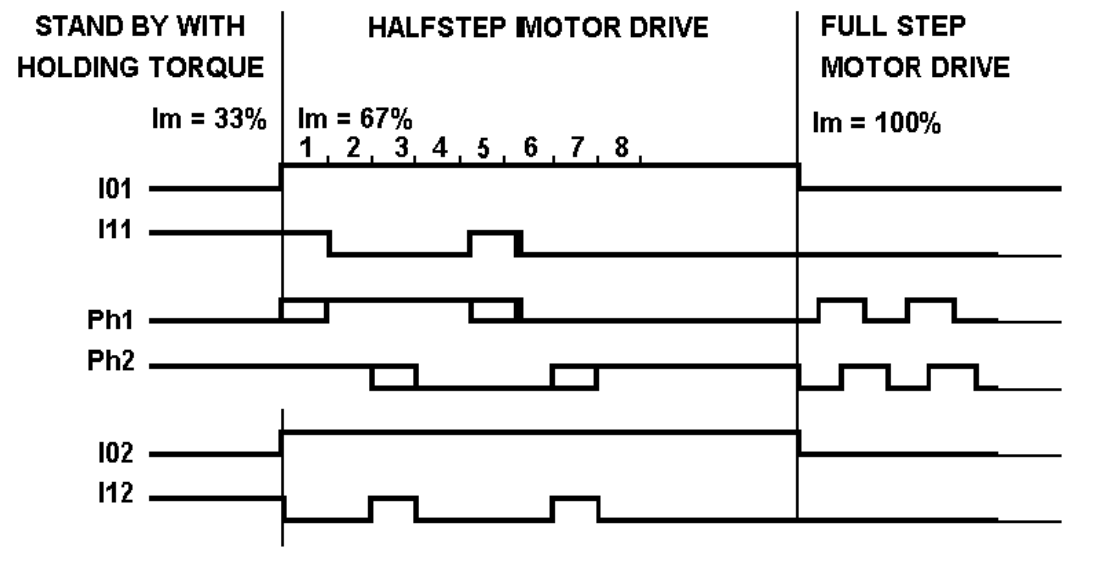
\includegraphics[width=0.55\textwidth]{stepperTiming}
  \caption{Stepper Motor Timing Diagram \cite{datasheet-L6219}}
  \label{fig:stepperTiming}
\end{figure}

The motors were setup in half-stepping mode at maximum current, as shown in Figure \ref{fig:stepperTiming}. The step sequence (as in the driver datasheet \cite{datasheet-L6219}) was implemented using an array. Since both axes on the mount are dependent (i.e. connected via Gear E) the two-axis mount requires some relatively involved control. Elevational variation is straight-forward, as the azimuthal motor (controlled by Gear C in Figure \ref{fig:antennaMount}) can be held fixed, and the elevation motor (Gear D) stepped accordingly. For azimuthal variation, if the elevation motor is held fixed, rotating the azimuthal motor causes the mount to also change in elevation, which must be compensated (demonstrated in Appendix \ref{sec:appendix_mount_rotation}). The ``azel" ratio is the number of elevation motor turns required to tilt the elevation axis the same amount as the azimuthal motor, given by:

\begin{equation}\label{eqn:azelRatio}
\textnormal{azelRatio} = \frac{D_{\textnormal{outer}} / B}{C / A} = \frac{92 / 20}{60 / 15} = 1.15
\end{equation}

\noindent The azimuthal and elevation angles can then be calculated as in Formulae \ref{eqn:azAngle} and \ref{eqn:elAngle}, where \textit{elRev} and \textit{azRev} are the number of elevation/azimuth motor steps per full revolution (equal to $200 \times \frac{92}{20} \times \frac{140}{80} = 1610$ and $200 \times \frac{60}{15} = 800$ respectively).
\begin{align}
    \textnormal{azAngle} &= \textnormal{azPos} \times \frac{360 ^{\circ}}{\textnormal{azRev}} \label{eqn:azAngle} \\
    \textnormal{elAngle} &= (\textnormal{azPos} \times \textnormal{azelRatio} + \textnormal{elPos}) \times \frac{360 ^{\circ}}{\textnormal{elRev}} \label{eqn:elAngle}
\end{align}

\noindent The number of simultaneous \textit{"delta"} steps to make in order for each axis to move to a new location \{\textit{newAzAng}, \textit{newElAng}\} implemented in \textit{setAzimuthElevation()} is then given by Formulae \ref{eqn:deltaAzSteps} and \ref{eqn:deltaElSteps}. Then, to smoothly step both motors simultaneously, speeds are set according to the ratio \textit{deltaAzSteps} : \textit{deltaELSteps}. A conversion from cartesian to azimuthal-elevation is then done to allow a boresight vector as input.
\begin{align}
    \textnormal{deltaAzSteps} &= \textnormal{angToPosAz(newAzAng)} - \textnormal{azPos} \label{eqn:deltaAzSteps} \\ 
    \textnormal{deltaElSteps} &= \textnormal{-deltaAzSteps} \times \textnormal{azelRatio} + \textnormal {angToPosDeltaEl(newElAng - elAng)}\label{eqn:deltaElSteps} 
\end{align}

\subsection{Pointing}
A small C++ header-only library titled \textit{wgs84} was used for the Mercator projection, with Cape Town as the origin. This allows a pointing vector to be determined, which could be set as the mount's boresight. Unfortunately, the purchased IMU (the MPU-9250) was found to be counterfeit and did not include a magnetometer. A constraint was therefore made that a dead-reckoning fix to face magnetic north should be done for the ground station. The angle between the zero sensor and magnetic north was therefore used as a reference input.

\subsection{Radio and GPS}
Existing Arduino libraries were wrapped into "cover classes", with the library \textit{Radiolib} initially being used for communication with the LoRa module. However, it was found that its implementation was too large in program size for the Atmega328. It was therefore replaced with an smaller implementation, \textit{LoRaLib}. For the GPS, \textit{TinyGPSPlus} was used.